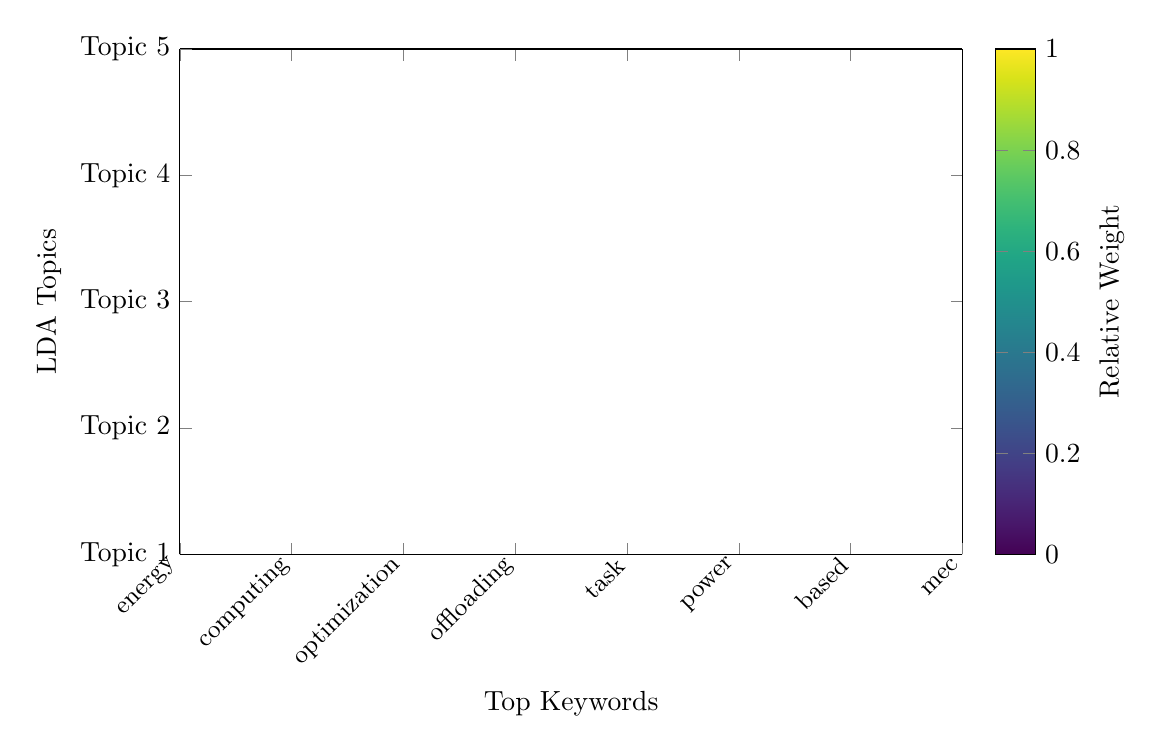
\begin{tikzpicture}
    \begin{axis}[
        colormap/viridis,
        colorbar,
        colorbar style={
            ylabel={Relative Weight},
        },
        width=0.95\textwidth,
        height=8cm,
        xlabel={Top Keywords},
        ylabel={LDA Topics},
        xtick={0, 1, 2, 3, 4, 5, 6, 7},
        xticklabels={energy, computing, optimization, offloading, task, power, based, mec},
        xticklabel style={rotate=45, anchor=east, font=\small},
        ytick={0, 1, 2, 3, 4},
        yticklabels={Topic 1, Topic 2, Topic 3, Topic 4, Topic 5},
        point meta min=0,
        point meta max=1,
        enlargelimits=false,
        axis on top,
        view={0}{90},
    ]

        \addplot3[
            surf,
            shader=flat,
            mesh/rows=5,
            mesh/cols=8,
            point meta=explicit,
        ] coordinates {
        (0,0,1.000)
        (1,0,0.556)
        (2,0,0.442)
        (3,0,0.369)
        (4,0,0.364)
        (5,0,0.312)
        (6,0,0.280)
        (7,0,0.280)
        (0,1,1.000)
        (1,1,0.725)
        (2,1,0.617)
        (3,1,0.596)
        (4,1,0.496)
        (5,1,0.479)
        (6,1,0.475)
        (7,1,0.466)
        (0,2,1.000)
        (1,2,0.926)
        (2,2,0.681)
        (3,2,0.584)
        (4,2,0.487)
        (5,2,0.476)
        (6,2,0.393)
        (7,2,0.385)
        (0,3,1.000)
        (1,3,0.386)
        (2,3,0.253)
        (3,3,0.205)
        (4,3,0.161)
        (5,3,0.152)
        (6,3,0.140)
        (7,3,0.131)
        (0,4,1.000)
        (1,4,0.718)
        (2,4,0.508)
        (3,4,0.435)
        (4,4,0.427)
        (5,4,0.374)
        (6,4,0.318)
        (7,4,0.276)
        };

    \end{axis}
\end{tikzpicture}